\section{Application Experience}\label{sec:application}

The application experience focus on supporting the user in a building modeling task. The exploited modeling approach requires the user to face as much as possible a bidimensional interface which allows her to define the floorplan and to place complex architectural elements (here called \emph{building elements}) on it. Such \emph{building elements} can be found in a pre-filled catalog, and when required can be further configured and customized through a side panel. This modeling approach move part of the complexity toward the developer of the customizable building elements, leaving to the final user the task to place and to configure the employed elements. A rich catalog of elements is thus crucial to answer to the users' modeling requirements.

Once the floorplan has been defined according to the \emph{place-and-configure} approach, the system can automatically generate a 3D model which can be explored externally or in first person view, as shown in Figure~\ref{FIGURA_IN_PRIMA_PERSONA}. Each  \emph{building element} in fact comprises either a \emph{2D generating function} than a \emph{3D generating function}, used to obtain models respectively used in the 2D floorplan definition and in 3D generated model.

The tool also has support for layers the user can exploit to organize her project, for example to group together semantically homogenous elements.

\subsection{Building Elements}\label{ssec:elements}

Along with the aforementioned 2D and 3D generating functions, an elements is fully specified by its univocal name and its properties, used by the user for customization. Each building element inherits from its \emph{prototype} (one and only one). In the prototype are mapped both the inherent characteristics and user interactions needed to add the element to the project and/or configure it.

The catalog comprises then four different types of elements:\\\\
\noindent \emph{Lines}. An element which belongs to this category is drawn selecting a start point and an end point. To move it one can drags one of the end point or can drags the entire line. An example: a \emph{wall}.\\\\
\noindent \emph{Openings}. An opening is an element that is linked to an element of the \emph{line} type, making an hole on it. The user create a new opening by dragging on a chosen line. Examples are \emph{doors} and \emph{windows}.\\\\
\noindent \emph{Areas}. An area is an element which is normally generated by insertion of the boundary vertices. For example a room basement is an area. In this case it is automatically generated from the lines representing walls, thanks to an algorithm which looks for closed cycles. The algorithm is composed by the following phases: (i) search of biconnected component by mean of Hopcroft-Tarjan algorithm~(see \cite{Hopcroft:1973:AEA:362248.362272}); (ii) removal of edges that are not part of a biconnected component; (iii) search of all cycles through an algorithm that do a double check of each edges sorted by angle; (iv) search of maximal cycles correspondent to perimeter edges by an application of Gauss's area formula; (v) removal of maximal cycles.\\\\
\noindent \emph{Object}. An element that is freely inserted into space with a drag and drop interaction is an object. Examples are tables and chairs.\\\

% The internal representation for Line types (e.g. walls) is undirected graph: each node maps coordinates of one tip of the line, each edge represents topological adjacency between vertex. This internal representation helps us to provide a drag and drop interaction for this element type, in fact each drag is performed by means of a relocation od a node that cause, other that the displacement of the requested wall, a displacement of each adjacent wall.


% Areas are automatically generated thanks to an analysis of the wall graph. The algorithm is composed by the following phases: (i) search of biconnected component by mean of Hopcroft-Tarjan algorithm~(see \cite{Hopcroft:1973:AEA:362248.362272}); (ii) removal of edges that are not part of a biconnected component; (iii) search of all cycles through an algorithm that do a double check of each edges sorted by angle; (iv) search of maximal cycles correspondent to perimeter edges by an application of Gauss's area formula; (v) removal of maximal cycles;


MA COME SI FA A PARLARE DI LINES SE POI LE AREE SONO DEFINITE DAI WALLS?? DANILO SE TROVI UNA SPIEGAZIONE LOGICA TENIAMO LINES ALTRIMENTI SIAMO OBBLIGATI A CAMBIARE IN WALLS.----- COS\`I VA MEGLIO?? QUESTA ERA LA PRIMA VERSIONE DELLE AREE MA NON \`E PI\`U STATA IMPLEMENTATA


\subsection{User Interface}\label{ssec:ui}

\begin{figure}[htb]
\centering
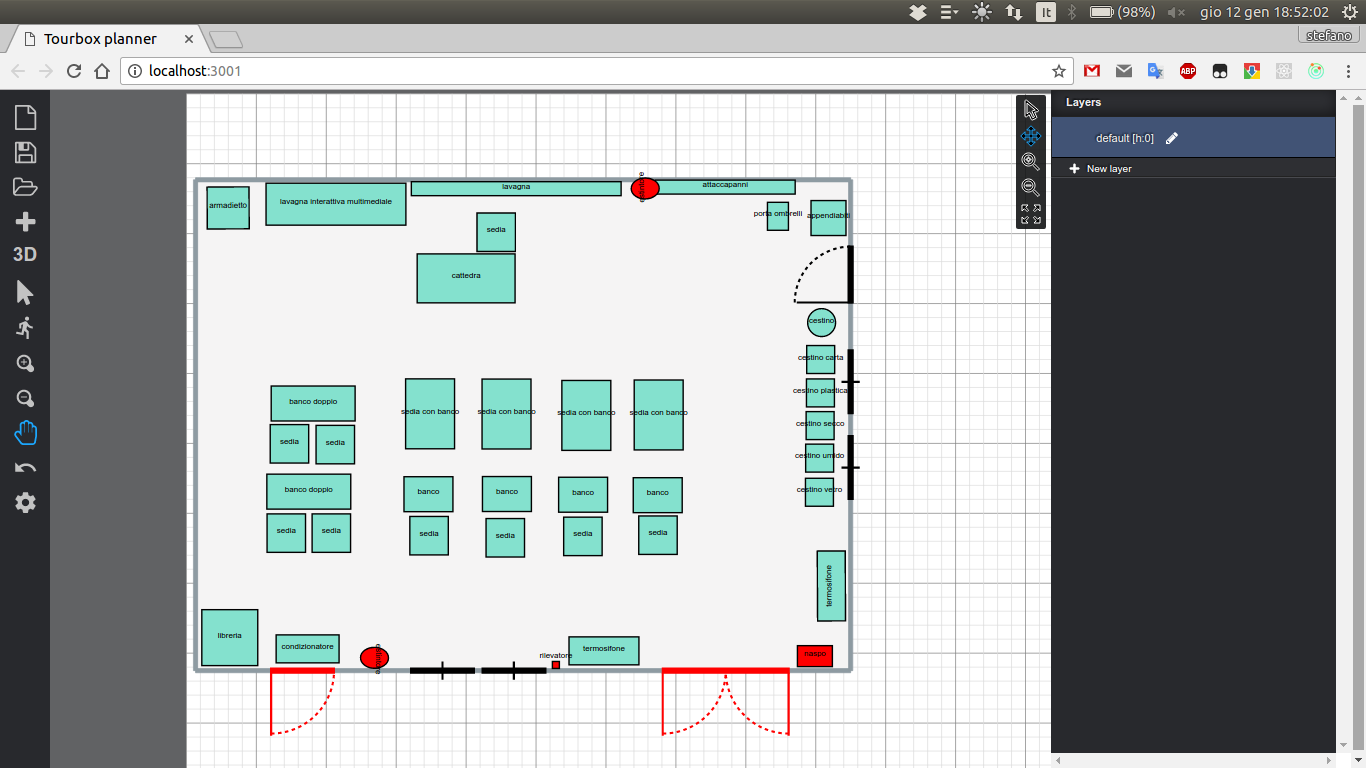
\includegraphics[width=\linewidth]{contents/images/fig2d}
\caption{The user interface}
\label{fig2D}
\end{figure}

Figure~\ref{fig2D} show the application user interface. It consists of the following components (from \textit{left} to \textit{right}):

\textbf{Toolbar:} it contains the button buttons mapping all operations the user can do in that context

\textbf{Content area}: it displays the main content requested by the user. In figure~\ref{fig2D} the content area shows the 2D drawing area.

\textbf{Sidebar:} it contains all elements in the current layer, the layer list and the properties for the selected building element\\

\begin{figure}[htb]
\centering
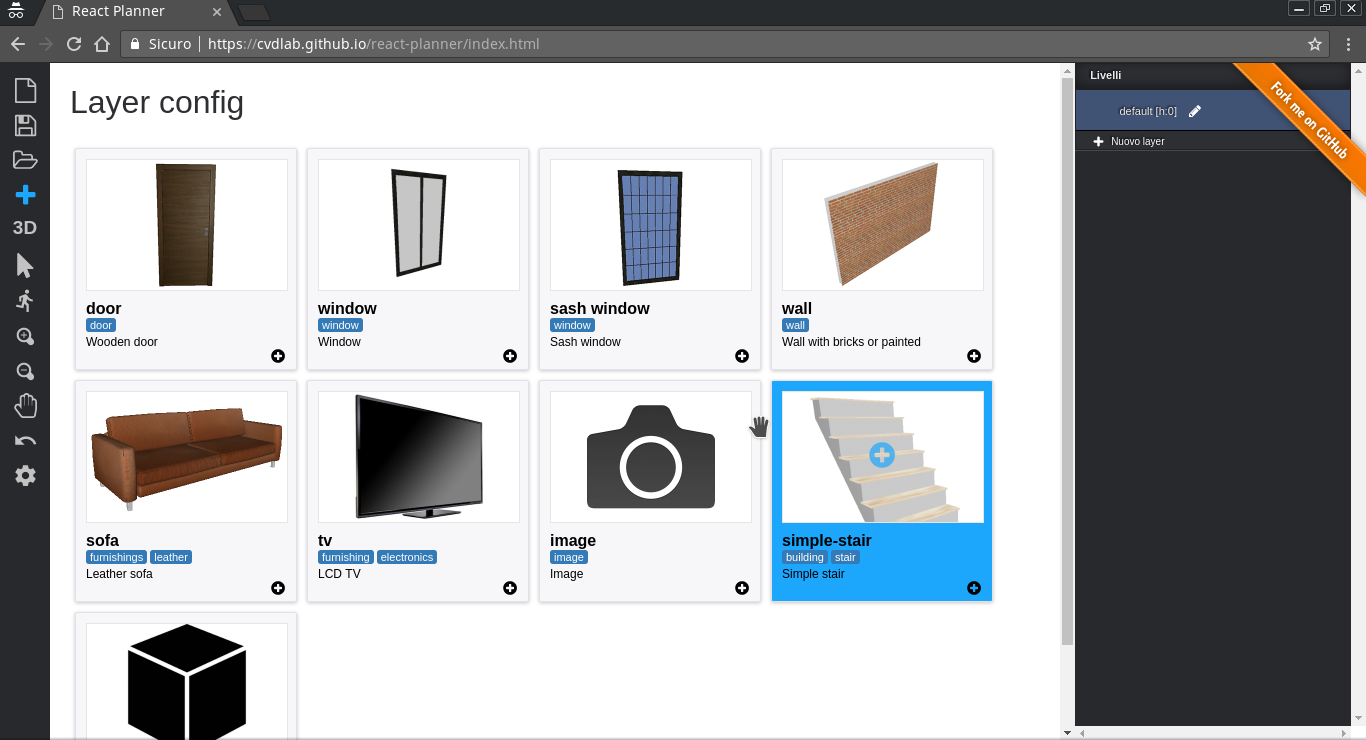
\includegraphics[width=\linewidth]{contents/images/figcatalog}
\caption{The building elements catalog}
\label{figCatalogo}
\end{figure}


Figure~\ref{figCatalogo} shows the building element catalog. When the user select one of the boxes, the application shows the 2D area and starts the interaction for the chosen building element.

\begin{figure}[htb]
\centering
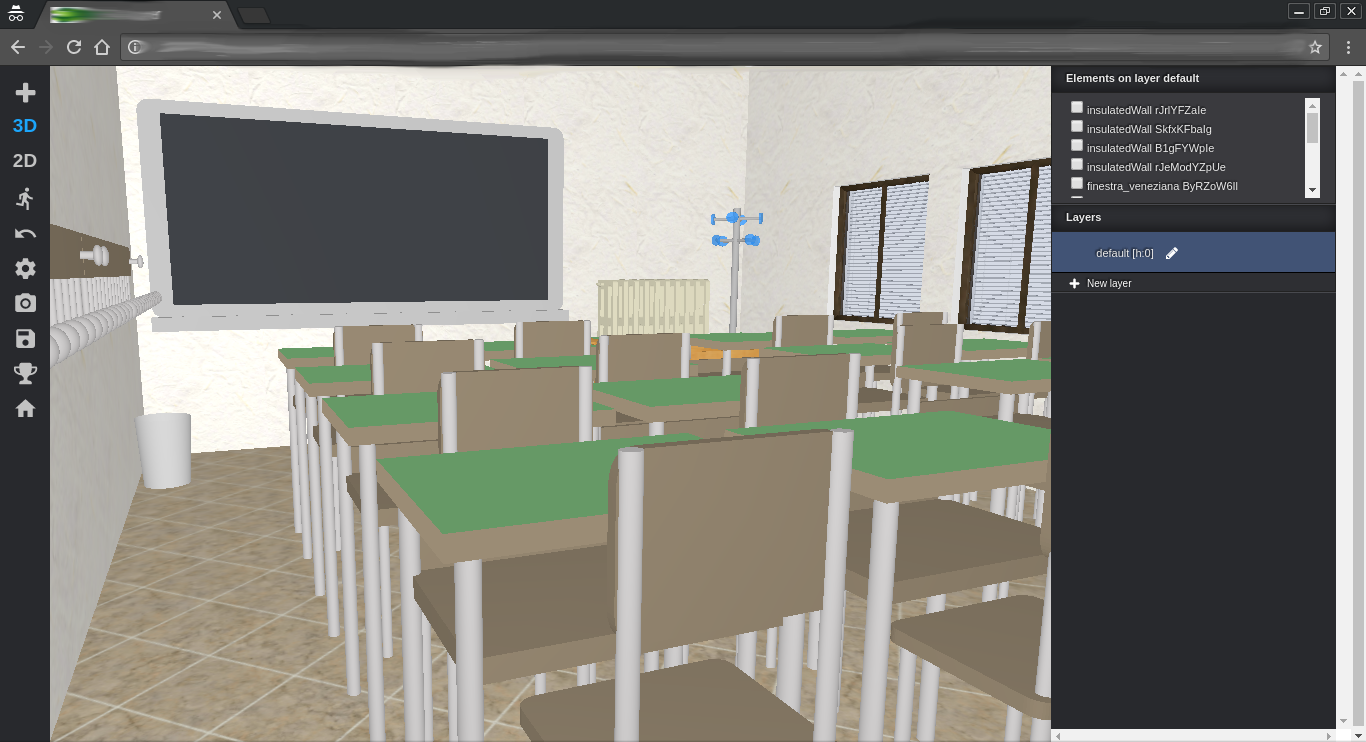
\includegraphics[width=\linewidth]{contents/images/3d-school}
\caption{3D visualization of a school}
\label{fig3D-school}
\end{figure}

\begin{figure}[htb]
\centering
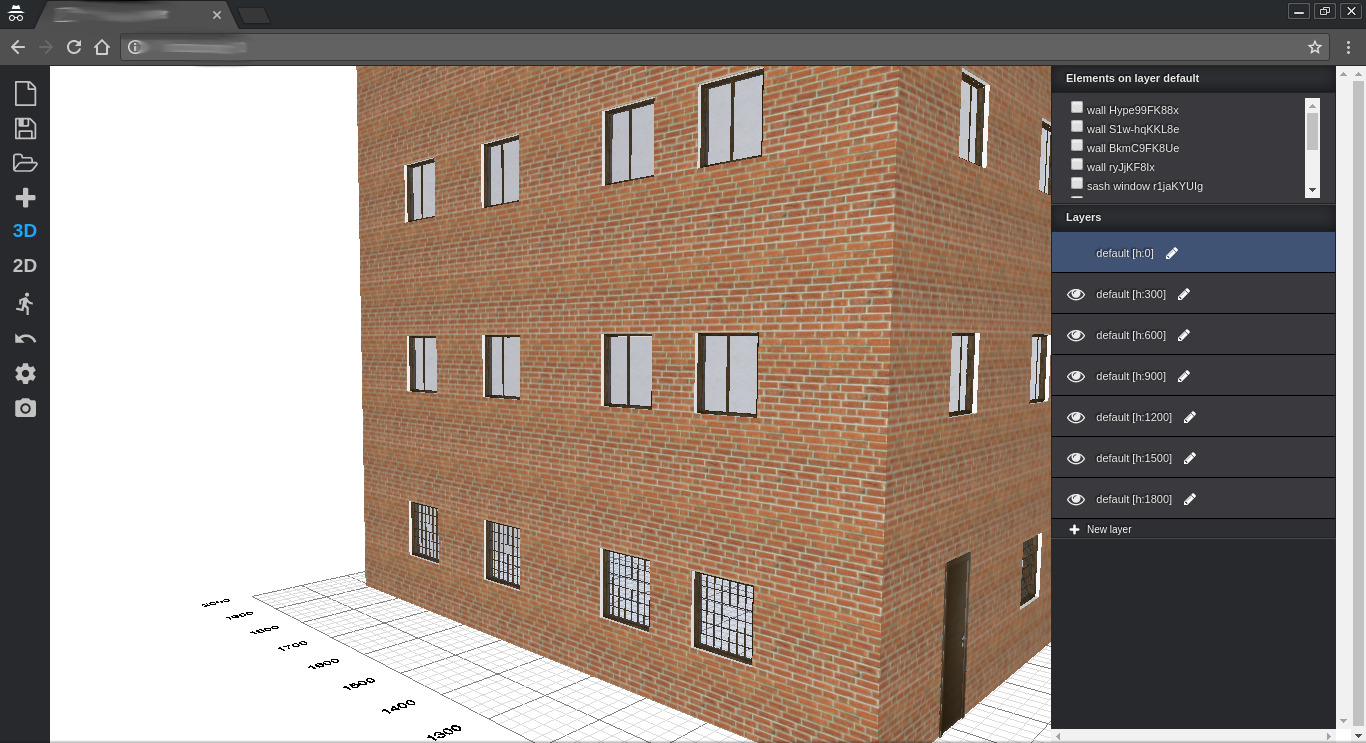
\includegraphics[width=\linewidth]{contents/images/palazzo2}
\caption{3D visualization of a building}
\label{fig3D-palace}
\end{figure}

Figures~\ref{fig3D-school} and~\ref{fig3D-palace} shows some examples of 3D visualizations.
